\documentclass[hidelinks, a4paper, 11pt]{scrartcl}

% Use-Packages:
\usepackage{graphicx}
\usepackage{color}
\usepackage{hyperref}
\usepackage{enumerate}
\usepackage{fontspec}
\setmainfont{Verdana}
\usepackage{pdflscape}

% Defined short commands please here
\def\app{``Telesales GUI''}
\def\com #1{\textcolor{red}{#1}}

% Headings
\pagestyle{myheadings}
\markright{Project: \app}

\makeatletter

\author{Rashad Asgarbayli}

\title{\vspace{3cm}
%
\includegraphics[scale=0.7]{Logo.png}\\
\app\vspace{20mm}}

\subtitle{Functional Specifications Document}

\date{\today}

\begin{document}

\maketitle
\thispagestyle{empty}

\newpage

\pagenumbering{roman}
\tableofcontents

\newpage

\pagenumbering{arabic}

\section{Introduction}

\paragraph{}We already have a batch tool named Telesales, that starts and runs automatic tests. But to configure the tool to run and do its work correctly, is more complexer. Because a co-worker needs minimum XML knowledge to create a right XML-Configuration file, and he/she has to do this manually. We need an application part, a GUI to make our configuration file faster and correct.
\paragraph{}Introducing a new Java(FX)-based GUI tool - \app{} for our batch application. \app{} will help You to create XML-Configuration files in an instant, thanks to its user-friendly interface and XML-creator engine. The co-worker only needs to enter some core data that needed for the batch-application. \app{} will than analyze the inputted data in the fields and generate a matching XML-Configuration files.

\newpage
\section{Objectives}

\paragraph{}Blablabla

\subsection{Mandatory Criteria}

\begin{itemize}
\item Blablabla
\item Blablabla
\item Blablabla
\end{itemize}

\subsection{Facultative Criteria}

\begin{itemize}
\item Blablabla
\item Blablabla
\item Blablabla
\end{itemize}

\subsection{Excluded Criteria}

\begin{itemize}
\item Blablabla
\item Blablabla
\item Blablabla
\end{itemize}


\newpage
\section{Product Usage}
   This section of the requirements is about the user groups of the system. It will be described how, why and by whom the \app will be used. 

\subsection{Blablabla}
\paragraph{}Blablabla

\subsection{Blablabla}
\paragraph{}Blablabla


\section{Product Environment}
\subsection{Environment for \app{}}
\paragraph{}\app{} is a Java (JavaFX) based application. Because of the java nature, it will run on all major OS's (Windows, Mac OS X, Linux etc.) as long as Java Runtime libraries installed. The minimum required Java runtime environment (JRE) is v1.8 (v8) or higher.

\subsection{Hardware}
\paragraph{}Minimum System Requirements depends of the minimum system requirements of Java and JavaFX.


\newpage
\section{Functional Requirements}

\subsection{Mandatory Functional Requirements}
\begin{description}
\item[/MF010/ Blablabla]\hfill \\ Blablabla
\item[/MF020/ Blablabla]\hfill \\ Blablabla
\end{description}

\subsection{Facultative Functional Requirements}
\begin{description}
\item[/FF010/ Blablabla]\hfill \\ Blablabla
\item[/FF020/ Blablabla]\hfill \\ Blablabla
\end{description}

\newpage
\section{Product Data}

\subsection{Essential data}
\begin{description}
\item[/D010/ BlaBlaBla]\hfill \\ Blablabla
\item[/D020/ BlaBlaBla]\hfill \\ Blablabla
\item[/D030/ BlaBlaBla]\hfill \\ Blablabla
\end{description}

\subsection{Facultative data}
\begin{description}
\item[/D010/ BlaBlaBla]\hfill \\ Blablabla
\item[/D020/ BlaBlaBla]\hfill \\ Blablabla
\item[/D030/ BlaBlaBla]\hfill \\ Blablabla
\end{description}


\section{Nonfunctional Requirements}

\begin{description}
\item[/NF010/ Bigger GUI Elements]\hfill \\ Bigger GUI elements provides better readability and makes it easy to work on touchscreen devices.
\end{description}

\newpage
\section{Global Test Cases and Scenarios}

In this section we describe the tests for the functional requirements in steps and with the wanted outcome. 

\subsection{Basic features}
\begin{description}
\item[/TB010/ BlaBlaBla]\hfill \\ Blablabla
\item[/TB020/ BlaBlaBla]\hfill \\ Blablabla
\item[/TB030/ BlaBlaBla]\hfill \\ Blablabla
\end{description}

\subsection{Optional features}
\begin{description}
\item[/TO010/ BlaBlaBla]\hfill \\ Blablabla
\item[/TO020/ BlaBlaBla]\hfill \\ Blablabla
\item[/TO030/ BlaBlaBla]\hfill \\ Blablabla
\end{description}

\newpage
\section{System Model}

\begin{figure}[h!]
\centering
%\includegraphics[width=0.8\textwidth]{mvc.png}
\caption{System Model}
\end{figure}

\paragraph{}The main model applied to the product is the
model-view-controller (MVC model).

\paragraph{}Blablabla

\subsection{Graphical User Interface}

\paragraph{}GUI is created using JavaFX 2 technology. It responds quite faster and easily  extendable.

\begin{figure}[h!]
\centering
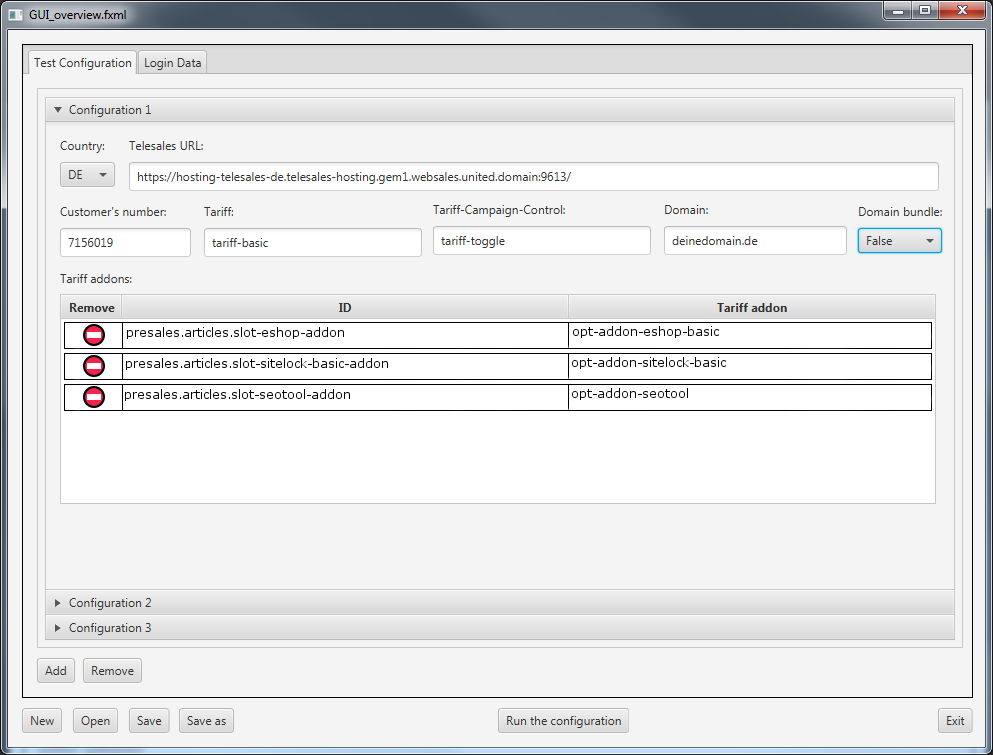
\includegraphics[width=\textwidth]{gui_batch_de.png}
\caption{View of the Configuration pane \textit{(Example configuration for the Germany)}}
\end{figure}

\begin{figure}[h!]
\centering
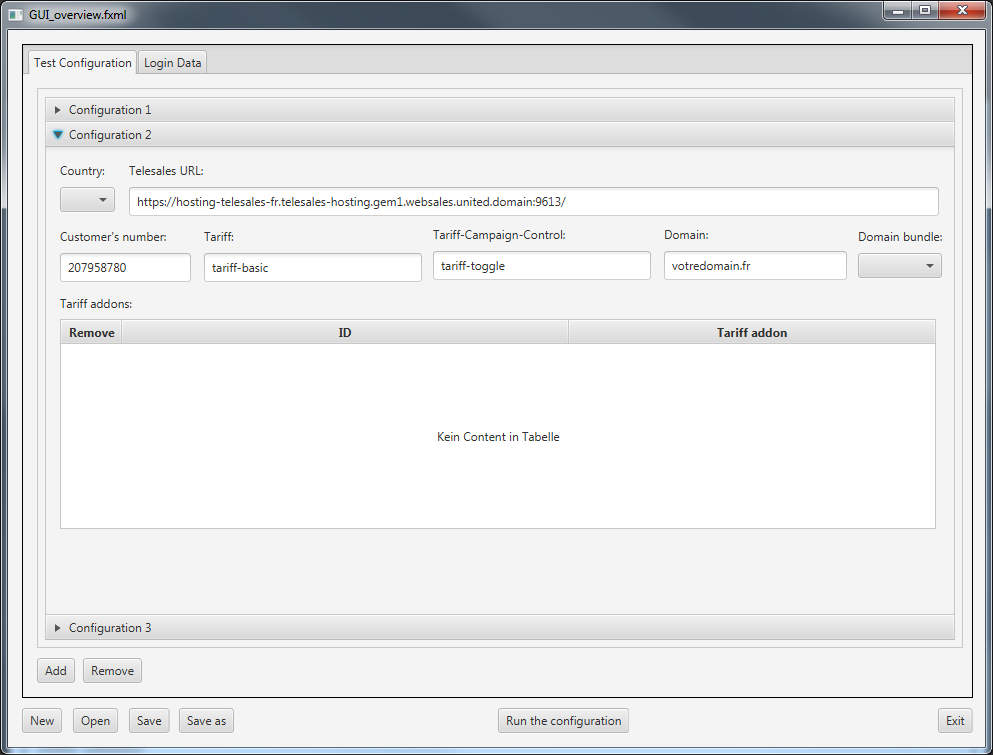
\includegraphics[width=\textwidth]{gui_batch_fr.png}
\caption{View of the Configuration pane \textit{(Example configuration for the France)}}
\end{figure}

\begin{figure}[h!]
\centering
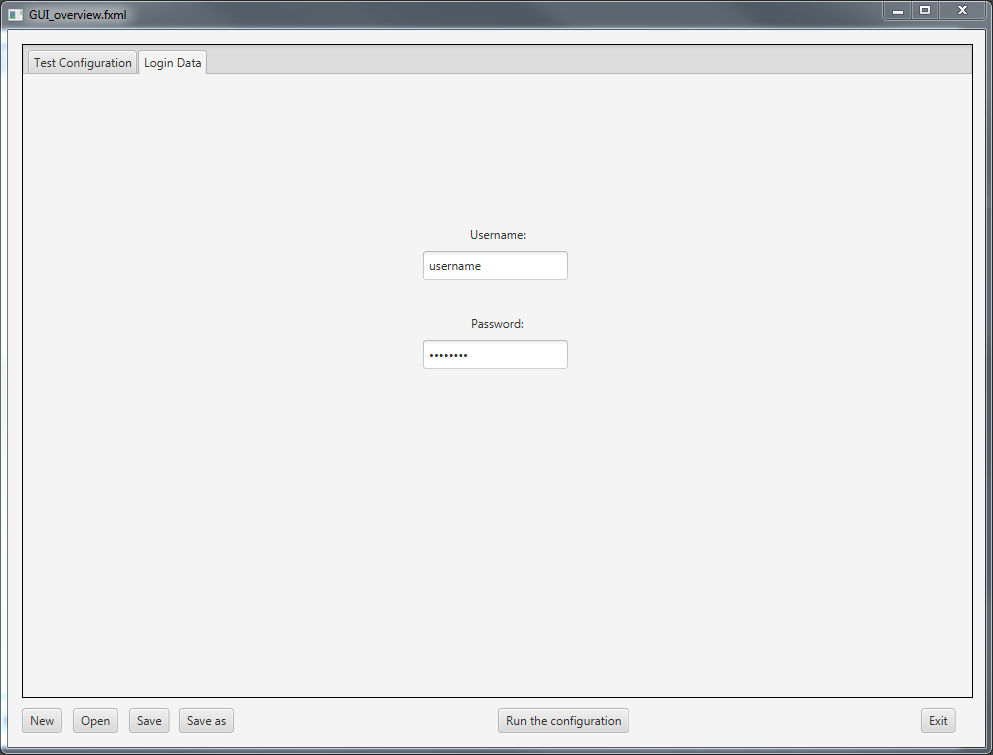
\includegraphics[width=\textwidth]{gui_login.png}
\caption{View of the login-data pane}
\end{figure}


\newpage
\section{Glossary}

\begin{description}
\item[GUI]\hfill \\ Graphical User Interface
\item[QA]\hfill \\ Quality Assurance
\item[User]\hfill \\ Co-worker of the QA
\end{description}

\end{document}
